% Options for packages loaded elsewhere
\PassOptionsToPackage{unicode}{hyperref}
\PassOptionsToPackage{hyphens}{url}
\PassOptionsToPackage{dvipsnames,svgnames,x11names}{xcolor}
%
\documentclass[
  letterpaper,
  DIV=11,
  numbers=noendperiod]{scrartcl}

\usepackage{amsmath,amssymb}
\usepackage{lmodern}
\usepackage{iftex}
\ifPDFTeX
  \usepackage[T1]{fontenc}
  \usepackage[utf8]{inputenc}
  \usepackage{textcomp} % provide euro and other symbols
\else % if luatex or xetex
  \usepackage{unicode-math}
  \defaultfontfeatures{Scale=MatchLowercase}
  \defaultfontfeatures[\rmfamily]{Ligatures=TeX,Scale=1}
\fi
% Use upquote if available, for straight quotes in verbatim environments
\IfFileExists{upquote.sty}{\usepackage{upquote}}{}
\IfFileExists{microtype.sty}{% use microtype if available
  \usepackage[]{microtype}
  \UseMicrotypeSet[protrusion]{basicmath} % disable protrusion for tt fonts
}{}
\makeatletter
\@ifundefined{KOMAClassName}{% if non-KOMA class
  \IfFileExists{parskip.sty}{%
    \usepackage{parskip}
  }{% else
    \setlength{\parindent}{0pt}
    \setlength{\parskip}{6pt plus 2pt minus 1pt}}
}{% if KOMA class
  \KOMAoptions{parskip=half}}
\makeatother
\usepackage{xcolor}
\setlength{\emergencystretch}{3em} % prevent overfull lines
\setcounter{secnumdepth}{5}
% Make \paragraph and \subparagraph free-standing
\ifx\paragraph\undefined\else
  \let\oldparagraph\paragraph
  \renewcommand{\paragraph}[1]{\oldparagraph{#1}\mbox{}}
\fi
\ifx\subparagraph\undefined\else
  \let\oldsubparagraph\subparagraph
  \renewcommand{\subparagraph}[1]{\oldsubparagraph{#1}\mbox{}}
\fi


\providecommand{\tightlist}{%
  \setlength{\itemsep}{0pt}\setlength{\parskip}{0pt}}\usepackage{longtable,booktabs,array}
\usepackage{calc} % for calculating minipage widths
% Correct order of tables after \paragraph or \subparagraph
\usepackage{etoolbox}
\makeatletter
\patchcmd\longtable{\par}{\if@noskipsec\mbox{}\fi\par}{}{}
\makeatother
% Allow footnotes in longtable head/foot
\IfFileExists{footnotehyper.sty}{\usepackage{footnotehyper}}{\usepackage{footnote}}
\makesavenoteenv{longtable}
\usepackage{graphicx}
\makeatletter
\def\maxwidth{\ifdim\Gin@nat@width>\linewidth\linewidth\else\Gin@nat@width\fi}
\def\maxheight{\ifdim\Gin@nat@height>\textheight\textheight\else\Gin@nat@height\fi}
\makeatother
% Scale images if necessary, so that they will not overflow the page
% margins by default, and it is still possible to overwrite the defaults
% using explicit options in \includegraphics[width, height, ...]{}
\setkeys{Gin}{width=\maxwidth,height=\maxheight,keepaspectratio}
% Set default figure placement to htbp
\makeatletter
\def\fps@figure{htbp}
\makeatother
\newlength{\cslhangindent}
\setlength{\cslhangindent}{1.5em}
\newlength{\csllabelwidth}
\setlength{\csllabelwidth}{3em}
\newlength{\cslentryspacingunit} % times entry-spacing
\setlength{\cslentryspacingunit}{\parskip}
\newenvironment{CSLReferences}[2] % #1 hanging-ident, #2 entry spacing
 {% don't indent paragraphs
  \setlength{\parindent}{0pt}
  % turn on hanging indent if param 1 is 1
  \ifodd #1
  \let\oldpar\par
  \def\par{\hangindent=\cslhangindent\oldpar}
  \fi
  % set entry spacing
  \setlength{\parskip}{#2\cslentryspacingunit}
 }%
 {}
\usepackage{calc}
\newcommand{\CSLBlock}[1]{#1\hfill\break}
\newcommand{\CSLLeftMargin}[1]{\parbox[t]{\csllabelwidth}{#1}}
\newcommand{\CSLRightInline}[1]{\parbox[t]{\linewidth - \csllabelwidth}{#1}\break}
\newcommand{\CSLIndent}[1]{\hspace{\cslhangindent}#1}

\KOMAoption{captions}{tableheading}
\makeatletter
\makeatother
\makeatletter
\makeatother
\makeatletter
\@ifpackageloaded{caption}{}{\usepackage{caption}}
\AtBeginDocument{%
\ifdefined\contentsname
  \renewcommand*\contentsname{Table of contents}
\else
  \newcommand\contentsname{Table of contents}
\fi
\ifdefined\listfigurename
  \renewcommand*\listfigurename{List of Figures}
\else
  \newcommand\listfigurename{List of Figures}
\fi
\ifdefined\listtablename
  \renewcommand*\listtablename{List of Tables}
\else
  \newcommand\listtablename{List of Tables}
\fi
\ifdefined\figurename
  \renewcommand*\figurename{Figure}
\else
  \newcommand\figurename{Figure}
\fi
\ifdefined\tablename
  \renewcommand*\tablename{Table}
\else
  \newcommand\tablename{Table}
\fi
}
\@ifpackageloaded{float}{}{\usepackage{float}}
\floatstyle{ruled}
\@ifundefined{c@chapter}{\newfloat{codelisting}{h}{lop}}{\newfloat{codelisting}{h}{lop}[chapter]}
\floatname{codelisting}{Listing}
\newcommand*\listoflistings{\listof{codelisting}{List of Listings}}
\makeatother
\makeatletter
\@ifpackageloaded{caption}{}{\usepackage{caption}}
\@ifpackageloaded{subcaption}{}{\usepackage{subcaption}}
\makeatother
\makeatletter
\@ifpackageloaded{tcolorbox}{}{\usepackage[many]{tcolorbox}}
\makeatother
\makeatletter
\@ifundefined{shadecolor}{\definecolor{shadecolor}{rgb}{.97, .97, .97}}
\makeatother
\makeatletter
\makeatother
\ifLuaTeX
  \usepackage{selnolig}  % disable illegal ligatures
\fi
\IfFileExists{bookmark.sty}{\usepackage{bookmark}}{\usepackage{hyperref}}
\IfFileExists{xurl.sty}{\usepackage{xurl}}{} % add URL line breaks if available
\urlstyle{same} % disable monospaced font for URLs
\hypersetup{
  pdftitle={On the Chicken \& Egg Problem in Transportation Electrification},
  pdfauthor={Jason Hawkins Ph.D.; Nicholas Aldridge},
  colorlinks=true,
  linkcolor={blue},
  filecolor={Maroon},
  citecolor={Blue},
  urlcolor={Blue},
  pdfcreator={LaTeX via pandoc}}

\title{On the Chicken \& Egg Problem in Transportation Electrification}
\author{Jason Hawkins Ph.D. \and Nicholas Aldridge}
\date{}

\begin{document}
\maketitle
\begin{abstract}
The relationship between electric vehicle adoption and charging station
deployment is often discussed in the transportation field but seldom
examined formally. In this paper, we make use of publicly available
charging station installation data and purchased vehicle registration
data by county to examine this important question. We apply causal
inference methods to ascertain the phasing and causal relationship
between these two markets. Non-linear Granger causality tests suggest a
feedback relationship between vehicle adoption and charging station
installations, with neither market exhibiting a definitive temporal
lead. While we find that charging station investments are necessary for
vehicle adoption, they are insufficient to encourage the necessary
market penetration absent complementary policy. Non-parametric
dose-response modeling finds that electric vehicle adoption declines
with charging station penetration beyond 140 stations per 100,000
persons when controlling for confounding effects. We provide further
insights regarding equity in current charging station locations and
mediating relationships with other policy and social variables.
\end{abstract}
\ifdefined\Shaded\renewenvironment{Shaded}{\begin{tcolorbox}[breakable, enhanced, boxrule=0pt, sharp corners, borderline west={3pt}{0pt}{shadecolor}, frame hidden, interior hidden]}{\end{tcolorbox}}\fi

\hypertarget{introduction}{%
\section{INTRODUCTION}\label{introduction}}

Countries around the world are starting to take action to fight the
harmful effects of anthropogenic climate change. A focus for climate
scientists and policy makers alike is to reduce the amount of CO2 that
is emitted into the atmosphere. One of the largest contributors to CO2
emissions is the transportation system, which in the United States is
responsible for 29 percent of total CO2 emissions (EPA 2021). Emissions
are driven by the reliance on fossil fuel products as the primary
transportation fuel source. High greenhouse gas (GHG) emissions are
exacerbated by driving patterns in the United States, which tend to mean
longer travel distances than other countries (ITF 2021). The high
attribution of transportation sector GHG emissions to fossil fuels means
that vehicle electrification is widely regarded as a critical tool for
climate change mitigation (Musti and Kockelman 2011). Scenario analyses
find that aggressive targets are required to increase vehicle
electrification in the United States, with some plans coming close to
95\% of vehicles being electric by 2050 (Larson et al. 2021). Less
aggressive plans assume a 60\% 2050 electric vehicle market share.
Despite these findings, the pace of plug-in electric vehicles (PEVs)
adoption - defined as the combination of battery-electric and plug-in
electric hybrid vehicles - remains well below the necessary level to
mitigate climate change impacts.

Adoption is driven by a number of factors related to vehicle properties,
such as price, driving range and charging time, and by factors outside
of vehicles properties, such as consumer characteristics, fuel prices,
and government policy. Purchase price is one of the main factors that
influences consumers to purchase electric vehicles. When surveyed about
reason why they would choose to not purchase an EV, potential buyers
cited the price as the biggest deterrent (Hidrue et al. 2011). Other
research has found that drastically increasing vehicle battery size
while not changing the price did very little to persuade buyers to
purchase PEVs (Adepetu and Keshav 2017). The least influential factor
related directly to the vehicle properties is the charging time. One
analysis found that when charging time was reduced from 10 hours to 10
minutes, while changing no other factors, consumers were still more
likely to pick gas-powered cars (Hidrue et al. 2011).

There are many factors not directly related to electric vehicles that
are influential in increasing EV adoption. The strongest of these
factors is the price of fuel. One study finds that a 10 percent increase
in fuel prices could increase in the market share of hybrid vehicles by
as much as 90 percent (Diamond 2009). In addition to fuel prices, the
characteristics of consumers influences how electric vehicles are
adopted. Characteristics like age and education are among the most
significant predictors of how likely a person is to purchase an PEV
(Hidrue et al. 2011). Another non-vehicle factor is government policy.
Most government policy is targeted at reducing the price of PEVs, but it
can encompass many other strategies like creating a more robust charging
infrastructure (often termed electric vehicle supply equipment, or
EVSE), which is the focus of this paper.

The lack of EVSE is a significant barrier to widespread PEV adoption
(Sullivan and Taylor 2021). A common policy put forward to increase
electric vehicle adoption is a federal income tax credit for EV buyers.
However, spending similar amounts on increasing deployment of charging
stations could yield more effective results (Li et al. 2017).
Governments are starting to use this knowledge when drafting spending
policy; recently, the US federal government passed an infrastructure
bill that allocates roughly \$5 billion to creating a network of
charging stations (The White House 2022). The network of charging
stations setup by this spending will be placed along designated roads,
particularly the US Interstate System. We begin by defining the
relationship between PEV adoption and EVSE as an indirect network effect
problem. We then outline two frameworks for causal inference, which
provide complementary perspectives on the problem. These methods are
applied to the United States using data for the period 2012 to 2020. We
provide analysis results, policy conclusions, and outline future work on
this topic.

\hypertarget{the-electric-vehicle-and-charging-station-problem}{%
\section{THE ELECTRIC VEHICLE AND CHARGING STATION
PROBLEM}\label{the-electric-vehicle-and-charging-station-problem}}

Electric vehicle ownership is often referenced as exhibiting a ``chicken
and egg'' behavior arising from the supply and demand relationship.
Individual demand for electric vehicles is influenced by the available
charging stations supply. Consumers are unwilling to purchase vehicles
due to range anxiety and a perceived lack of charging stations.
Suppliers are not incentivized to provide charging stations unless there
is sufficient demand to warrant their cost. In more formal language, the
problem represents a indirect network effect. Similar dynamics exist in
other markets - e.g., consumers choose online streaming video services
based on their offerings, but service providers require capital from
subscriptions in order to generate content. There is a clear role for
public policy in such situations when a public good results from
intervention in the market. Many governments may deem PEVs as a solution
to a public ill (i.e., climate change) and can incentivize either
suppliers by providing installation subsidies or consumers by installing
charging stations. While the problem has been recognized in the
literature (Melliger, Vliet, and Liimatainen 2018), empirical analysis
is minimal.

Zhou and Li (Zhou and Li 2018) find that government spending on EVSE
deployment is most effective in the early stages of PEV market
penetration. These early markets may have critical-mass constraints,
which can be overcome by a government subsidy that deals with the
network effect. Subsidies for charging stations are found to be more
effective than those for PEV purchases because early PEV adopters have a
low-price sensitivity(Li et al. 2017). Early adopters are eager to
purchases PEVs, which makes them more willing to pay higher prices. The
main consumer concern at this stage is the ability to recharge their
vehicle - that is, the existing EVSE environment. Because of this,
understanding consumer's preferences for charging station infrastructure
is crucial. Sheldon et al. (Sheldon, DeShazo, and Carson 2019) find that
consumers are willing to pay about 5 cents per mile for plug-in electric
vehicles and about 10 cents per minute of wait time while refueling.
Consumers are also willing to wait up to 8 minutes longer during
refueling relative to the time for conventional fossil fuel vehicles.
Knowing this information can allow policy makers to create subsidy
programs that produce more effective outcomes.

An important feature when considering an electrified mobility system is
how its refueling infrastructure differs from the conventional fossil
fuel-based system. In the conventional private mobility system, the
individual owns the vehicle and purchases fuel from centralized and
privately owned refueling stations. These vehicles typically have a
greater driving range associated with them. While the increased range
increases a vehicle's mobility, refueling at a place of residence is not
viable. Electric vehicles do not have as great of a driving range as
gas-powered vehicles. However, electric vehicles may be charged in the
home using previously existing electrical infrastructure. The presence
of charging points in the home begs the questions 1) if (or to what
extent) out-of-home charging stations are required for travel, and 2) to
what extent is range anxiety a perception versus a reality.

According to the Bureau of Transportation Statistics, 98\% of trips made
in the US are less than 50 miles (Vehicle Technology Office 2022). Given
that most battery-electric vehicles (BEVs) have a range greater than 200
miles (Elfalan 2021), it is feasible to make most trips on a single
charge. However, long-distance trips (over 50 miles) comprise 30\% of
total vehicle-miles traveled (VMT) (Aultman-Hall 2018). There is clearly
a need for out-of-home charging stations to accommodate these trips.
Even if most trips can be accommodated by in-home charging, the vehicle
purchase decision will be influenced by consideration of these longer
trips that require charging stations (Silvia and Krause 2016).
Additionally, Wolbertus et al. (Wolbertus et al. 2018) find that there
is still a demand for charging stations in places where public daytime
charging is the only option, such as at the workplace.

We contribute to this literature by providing among the first and most
extensive examinations of the co-evolving PEV and EVSE systems. Zhou and
Li (Zhou and Li 2018) used data for 2011-2013 vehicle sales and EVSE for
353 US metropolitan aras, which we are able to expand to include a
longer time horizon (2012-2020) and wider spatial extent (all counties
in the United States). Further, we combine two causal inference
approaches to capture both the phasing and causal relationship between
these markets.

\hypertarget{methods}{%
\section{METHODS}\label{methods}}

We define two classes of causality which we termed as phasing causality
and potential outcomes causality. These alternative forms of causality
are often denoted by their principle developers: Granger causality
(Granger 1969) and Rubin causality (Rubin 2005), respectively. Both
approaches are employed due to the (functionally) continuous nature of
the two variables of interest. We detail each approach and its
application to the present problem below.

\hypertarget{non-linear-phasing-causality}{%
\subsection{Non-Linear Phasing
Causality}\label{non-linear-phasing-causality}}

Define two variables \(X_t\) and \(Y_t\) where subscript \(t\) denotes a
time series process. Phasing causality seeks to identify whether the two
time series exhibit a common pattern (or coherence). One variable may
lead the other producing a time lag, but the series may also exhibit
instantaneous \emph{causality} whereby the current value of \(Y_t\) is
better predicted when the current value of \(X_t\) is included in the
model. In strict terms, phasing causality is defined by
\[\sigma^2(Y|U)<\sigma(Y|\overline{U-X})\] \{\#eq:granger-causality\}.
There is also the potential for feedback, whereby \(X_t\) causes \(Y_t\)
and \(Y_t\) also causes \(X_t\). In the EV and charging station
situation, this might mean that EVSE installations encourage households
in a county to purchase PEVs, which then encourages further investment
in EVSE infrastructure. There are two key principles underling phasing
causality: 1) that the cause occurs before its effect and 2) that the
cause has unique information about the future values of its effect.
Granger defines a simple test statistic for such causality using time
series data using the F-test.

The original applications of Granger causality were to economic
variables that fluctuated over time. The test assumes that both \(X_t\)
and \(Y_t\) are stationary time series, an assumption that will be shown
to be violated in the present case. Several extensions have been
developed to phasing causality that allow for non-stationary time
series. We use the approach of Rosol et al. (Rosoł, Młyńczak, and
Cybulski 2022) with modifications to fit our application as detailed in
the following section. Their approach compares the model median absolute
error using both time series (\(Y_t\) and \(X_t\))to that obtained using
only the dependent time series (\(Y_t\)). The Wilcoxon signed-rank test
is used to test for statistical significance - i.e., that \(X_t\) causes
\(Y_t\). The method is implemented as a Python package and includes
multilayer perceptron (MLP), long short-term memory (LSTM), gated
recurrent unit (GRU), neural net (NN), and autoregressive integrated
moving average (ARIMA) models. Model errors are calculated at each
observation and the sum of their absolute values used in the statistical
test. The method has the ability to measure changes in causality over
time, but our time series is too short for its application.

\hypertarget{potential-outcomes-causality-via-propensity-score-matching}{%
\subsection{Potential Outcomes Causality Via Propensity Score
Matching}\label{potential-outcomes-causality-via-propensity-score-matching}}

Potential outcomes causality begins from the definition that causal
effects are a comparison between outcomes \(Y\) in response to
differences in a treatment \(T\) on a common set of units.
Unfortunately, such an analysis is not possible in reality since it
would require the same unit (e.g., person) to simultaneously experience
both the treated and untreated conditions. In observational studies, a
common approach is to identify two sets of observational units that
differ only in their exposure to a treatment variable of interest. A
study interested in the effect of a new teaching strategy might compare
two sets of schools that differ only in whether they adopted the
strategy. A class of strategies to identify otherwise similar
observational units (e.g., schools) is propensity score matching.
Formally, the assumption is that \(Y_t \perp T|X_t\), or that outcome
\(Y_t\) is independent of the treatment conditional upon a set of
\(X_t\) covariates. That is, treatment assignment is ignorable
conditional on \(X_t\). However, for the present problem the treatment
(i.e., charging stations) is not binary. An observation unit may have
any number of charging stations.

An extension to the standard propensity score, termed as generalized
propensity score (GPS) matching, was developed by Hirano and Imbens
(Hirano and Imbens 2005). Assuming a continuous treatment, the GPS is
defined by
\begin{equation}\protect\hypertarget{eq-gps}{}{r(t,x)=f_{T|X}(t|x)}\label{eq-gps}\end{equation}
where \(t\in \tau\) is referred to as the unit-level dose-response
function, \(X\) and \(T\) are random variables defined on a common
probability space, and \(r(t,x)\) is the GPS measure defining similarity
between observational units. It can then be stated that
\(X\perp 1{T=t}|r(t,X)\), or that assignment to a treatment value \(t\)
is independent conditional on its GPS.

The dose-response nomenclature is taken from pharmeutical research,
where the interest is in the health response to a continuous drug dose.
Each individual has a potential response at different doses, or
treatment levels. The dose-response function that is an outcome of
continuous GPS analysis is an average of the potential responses at each
treatment level - an average dose-response function (ADRF). A challenge
when transitioning from a binary to a continuous treatment is that a
treated unit will not be available at every treatment level. The problem
can be addressed by parameterizing the curve as a linear combination of
a finite number of basis functions (Galagate 2016). The averaging used
to construct the ADRF is based on weighting observations by the GPS
using units within each basis function range.

\hypertarget{casual-mediation}{%
\subsection{Casual Mediation}\label{casual-mediation}}

A secondary question is the potential relationship between charging
stations and other variables of interest. These relationships can be
illustrated via a directed acyclic graph (DAG) as shown in
Figure~\ref{fig-dag} where \(X\) is a treatment variable, \(Z\) is a
mediating variable, and \(Y\) is an outcome variable (Imai, Jain, and
Ching 2009).

\begin{figure}

{\centering 

\begin{figure}[H]

{\centering 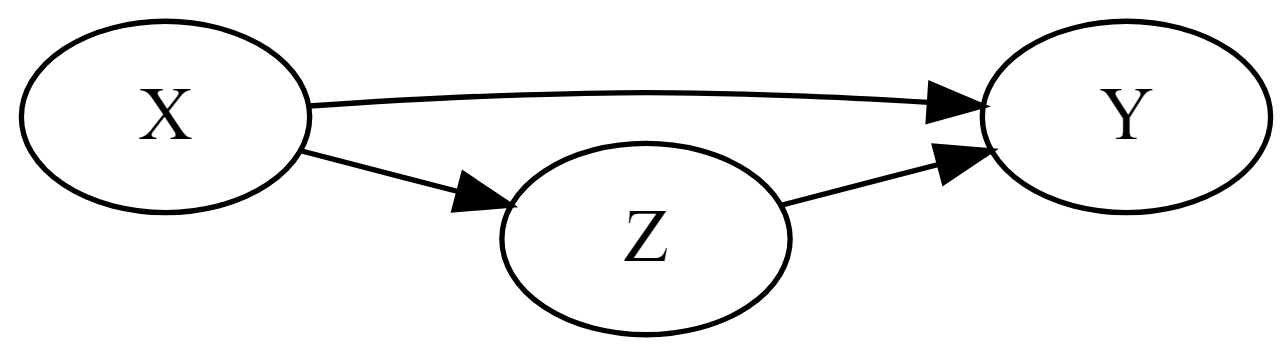
\includegraphics[width=2.52083in,height=0.69792in]{TRB_2023_files/figure-latex/dot-figure-1.png}

}

\end{figure}

}

\caption{\label{fig-dag}Directed Acyclic Graph (DAG) for Causal
Mediation}

\end{figure}

Conventional causal mediation modeling takes the form of a linear
structural equation model (SEM). Extending the above notation, \(M_t\)
is a mediation variable. Following the potential outcomes framework,
suppose we are interested in the mediating effect of EVSE investments on
grid decarbonization. In many cases, utility operators provide financial
support for EVSE. Limited budgets mean that a private firm or government
agency may need to balance investments in both infrastructures.
Previously, the potential outcome depended only on the treatment
variable but now depends on both the treatment and mediator variables as
\$Y(t,m)\$. Also, assume there is no interference effect meaning that
mediator values for one observation do not affect the treatment value
for other observations, and vice versa. The causal mediation (indirect)
effect for each observation is then given by
\begin{equation}\protect\hypertarget{eq-med}{}{\delta(t)=Y(t,M(1)-M(0)}\label{eq-med}\end{equation}
where \(M(1)\) and \(M(0)\) are the potential mediator variable values
with and without the treatment. The mediation effect is interpreted
based on the difference between \(M(1)\) and \(M(0)\) holding the
treatment fixed at \$t\$. If \(M(1)=M(0)\) - i.e., the treatment has no
effect on the mediator variable - then the causal mediation effect is
zero. Again, we use a generalized additive model (GAM) to test a
nonparametric average mediation effect.

\hypertarget{data-and-model-specification}{%
\section{DATA AND MODEL
SPECIFICATION}\label{data-and-model-specification}}

\hypertarget{treatment-and-outcome-variables}{%
\subsection{Treatment and Outcome
Variables}\label{treatment-and-outcome-variables}}

The two key input datasets are charging station locations provided by
the Alternative Fuel Data Center (AFDC) and electric vehicle
registrations provided by Experian Inc.~The vehicle registration dataset
comprises a 10-year panel at 2-year intervals (2012, 2014, 2016, 2018,
2020). Total vehicle registrations are recorded by county, make, model,
year, and other vehicle characteristics for the United States. The
frequency and spatial resolution of the vehicle registration data define
the analysis units. Our treatment and outcome variables are charging
stations and EV registrations normalized by population (per 100,000
persons).

Charging stations are geocoded and aggregated into annual cumulative
totals by county. Only public charging stations are maintained for
analysis. Further, the we make no distinction between charger port
capacity (level 1, 2, or 3) when aggregating the number of charging
ports per county. Such a distinction could be made as a sensitivity test
but may reduce the effective sample size as not all counties with
charging stations have all three charger port types.

After filtering out protectorates and other non-state locations, several
county codes in the Experian data remain that are missing registration
totals in a subset of years (117/3275, or about 4\%). We remove county
codes with more than one missing year, leaving 34 counties for which
registration totals are interpolated from adjacent years. Many of these
county codes are for remote areas with low populations (e.g., the
Aleutian Islands in Alaska). Of the 3140 viable counties, it is found
that 1406 lack EV registrations or public charging stations in any
analysis year. These counties are excluded from analysis because they
lack variation for model estimation. Figure~\ref{fig-missing}
illustrates that a further 80\% of the remaining counties did not have
EV registrations in 2012. While kept in the dataset for analysis, the
high proportion of zero-valued observations poses a significant
challenge for statistical inference.

\begin{figure}

\begin{minipage}[t]{\linewidth}

{\centering 

\raisebox{-\height}{

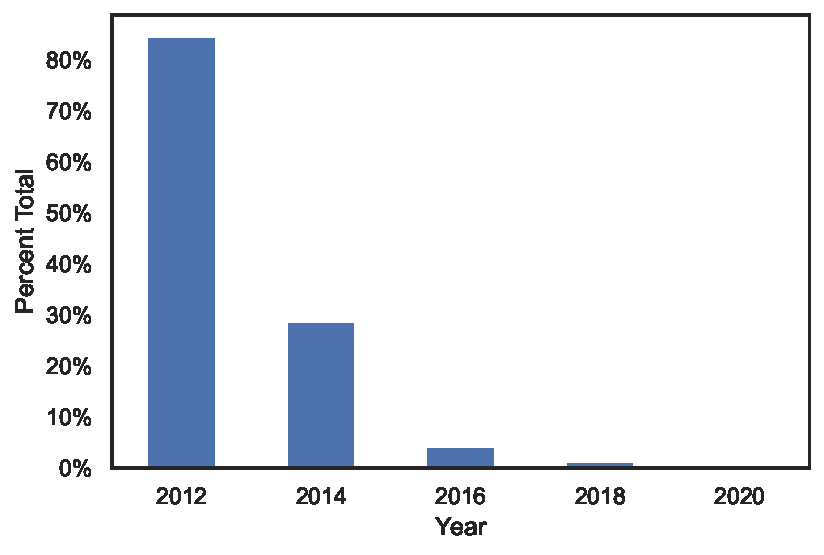
\includegraphics{TRB_2023_files/figure-pdf/fig-missing-output-1.pdf}

}

\caption{\label{fig-missing}Counties with no PEV registrations by year}

}

\end{minipage}%

\end{figure}

\hypertarget{covariates}{%
\subsection{Covariates}\label{covariates}}

Census data was compiled to construct county-level statistics for median
income and racial composition. Five-year American Community Survey (ACS)
data were used to approximate annual variation. We use the 2011-2015 ACS
for years 2012 and 2014 and the 2016-2020 ACS for years 2016, 2018, and
2020. For the purposes of analysis, we define minority racial groups as
Black and Hispanic based on an overrepresentation of poverty according
to Census Bureau analysis (US Census Bureau 2020). We also include
American Indian and Alaska native, and Native Hawaiian and Other Pacific
Island, and Other Race Not Specified in our definition.

To capture spatial spillover effects, a Queen contiguity matrix is
constructed for charging station density (per 100,000 persons) in
adjacent counties. The rationale is that an individual may purchase an
EV if there are charging stations in adjacent counties and charge at
their residence when driving in their home county. This specification is
termed a \emph{spatial lag in X} model in the spatial econometric
literature (Elhorst and Vega 2017)\emph{.}

Several studies (Sheldon, DeShazo, and Carson 2019; Li et al. 2017) find
that gas price at the pump is an important factor for PEV adoption. We
construct a fuel price variable using annual average prices for the
United States provided by the EIA (EIA 2022). We adjust these totals to
account for state variation using current state-level averages provided
by AAA (AAA 2022). Prices are then adjusted to 2020 dollar to ensure
consistent parameter inference.

\hypertarget{model-specification}{%
\subsection{Model Specification}\label{model-specification}}

We use the causal-curve Python package developed by Kobrosly (Kobrosly
2020) for potential outcomes causal inference. This package uses a
generalized linear model (GLM) to construct the GPS and a generalized
additive model (GAM) to estimate the dose-response curve. The GAM model
takes as inputs the GPS, a treatment grid, and a number of splines. We
use the default 100 unit grid and 30 splines (i.e., separating the GPS
space using 30 basis functions). The model includes state-year fixed
effects to account for unobserved policy variation and approxiamte
autocorrelation between observations for the same county. Extensions to
this model formulation are left for future work.

Causal mediation is explored for two variables. First, we consider the
mediating effect of EVSE on grid carbon intensity. We use state-level
eGrid data available for each analysis year. The treatment variable in
this case is state annual \(CO_2\) equivalent output emissions measured
in lbs per MWh. We hypothesize that public EVSE access may not be as
important to PEV adoption as perceived environmental benefit as measured
by grid emissions output intensity.

Second, we use 2020 county-level presidential election results as a
proxy for local political effects. Climate policies have been more
strongly pushed by Democratic presidential administrations, including
the recent legislation by the Biden Administration to support PEV
charging station infrastructure. Climate policy is also set at the
state-level, so gubernatorial election returns are an alternative
political variable. However, consistent county-level data were not
readily available from a single source. The causal hypothesis is that
political affiliation is associated with a proclivity towards
environmentally considerations when purchasing a vehicle. A change in
EVSE access is a mediating variable on higher Democratic affiliation (as
a proxy for public sentiments about the need for climate change action)
leading to PEV adoption.

\hypertarget{results}{%
\section{Results}\label{results}}

\hypertarget{descriptive-analysis}{%
\subsection{Descriptive Analysis}\label{descriptive-analysis}}

@fig-us-totals provides a first validation of the research hypothesis
that there is a relationship between PEV adoption and EVSE access.
Registered PEVs and public charging stations are normalized by
population and plotted over the eight year analysis period for the
United States. The two infrastructure show a similar exponential
increase, suggesting there is a correlation between their adoption but
giving no indication of temporal phasing or causality. This initial plot
also ignores regional variations, which will be important to
understanding the drivers of the relationship.

\begin{figure}

\begin{minipage}[t]{\linewidth}

{\centering 

\raisebox{-\height}{

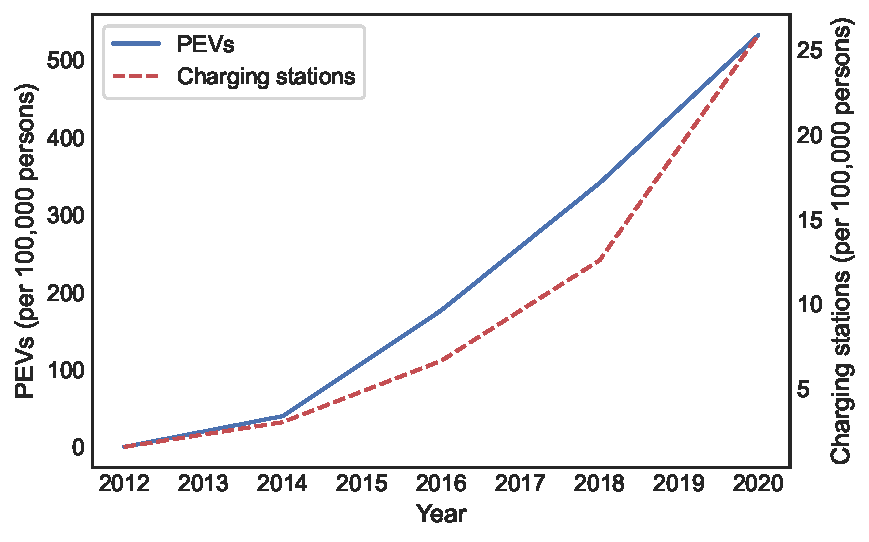
\includegraphics{TRB_2023_files/figure-pdf/fig-us-totals-output-1.pdf}

}

\caption{\label{fig-us-totals}US PEV registrations and charging stations
by year}

}

\end{minipage}%

\end{figure}

The Bipartisan Infrastructure Act places a strong focus on equitable
investment allocation. Equity can be explored both inter-regionally and
intra-regionally by key demographic features. @fig-equity compares the
distribution of charging stations for four representative cities. Omaha
is located in the central Great Plains, a region that has received
minimal exploration in the EV literature. Chicago and Detroit are large
cities with well-documented histories of housing segregation (Menendian,
Gambhir, and Hsu 2020). San Francisco is included as an example of a
large city in a progressive state. In all four cities, charging stations
are concentrated in the central city. San Francisco does not show clear
evidence of inequality, likely partially as a function of the overall
high density of charging stations. However, Chicago and Detroit both
show clear patterns of low charging station density in their
majority-minority communities and unexpectedly high station densities in
low density suburban communities. While there are few charging stations
in Omaha, those outside its downtown are located along an east-west axis
along the I-80 corridor. There are few stations in north and south
Omaha, which are enclaves of Black and Hispanic residents, respectively.
Similar inequities have been observed across US cities for other
transportation infrastructure investments, such as rail transit stations
that map more closely to income than population density (Spieler 2020).

\begin{figure}

{\centering 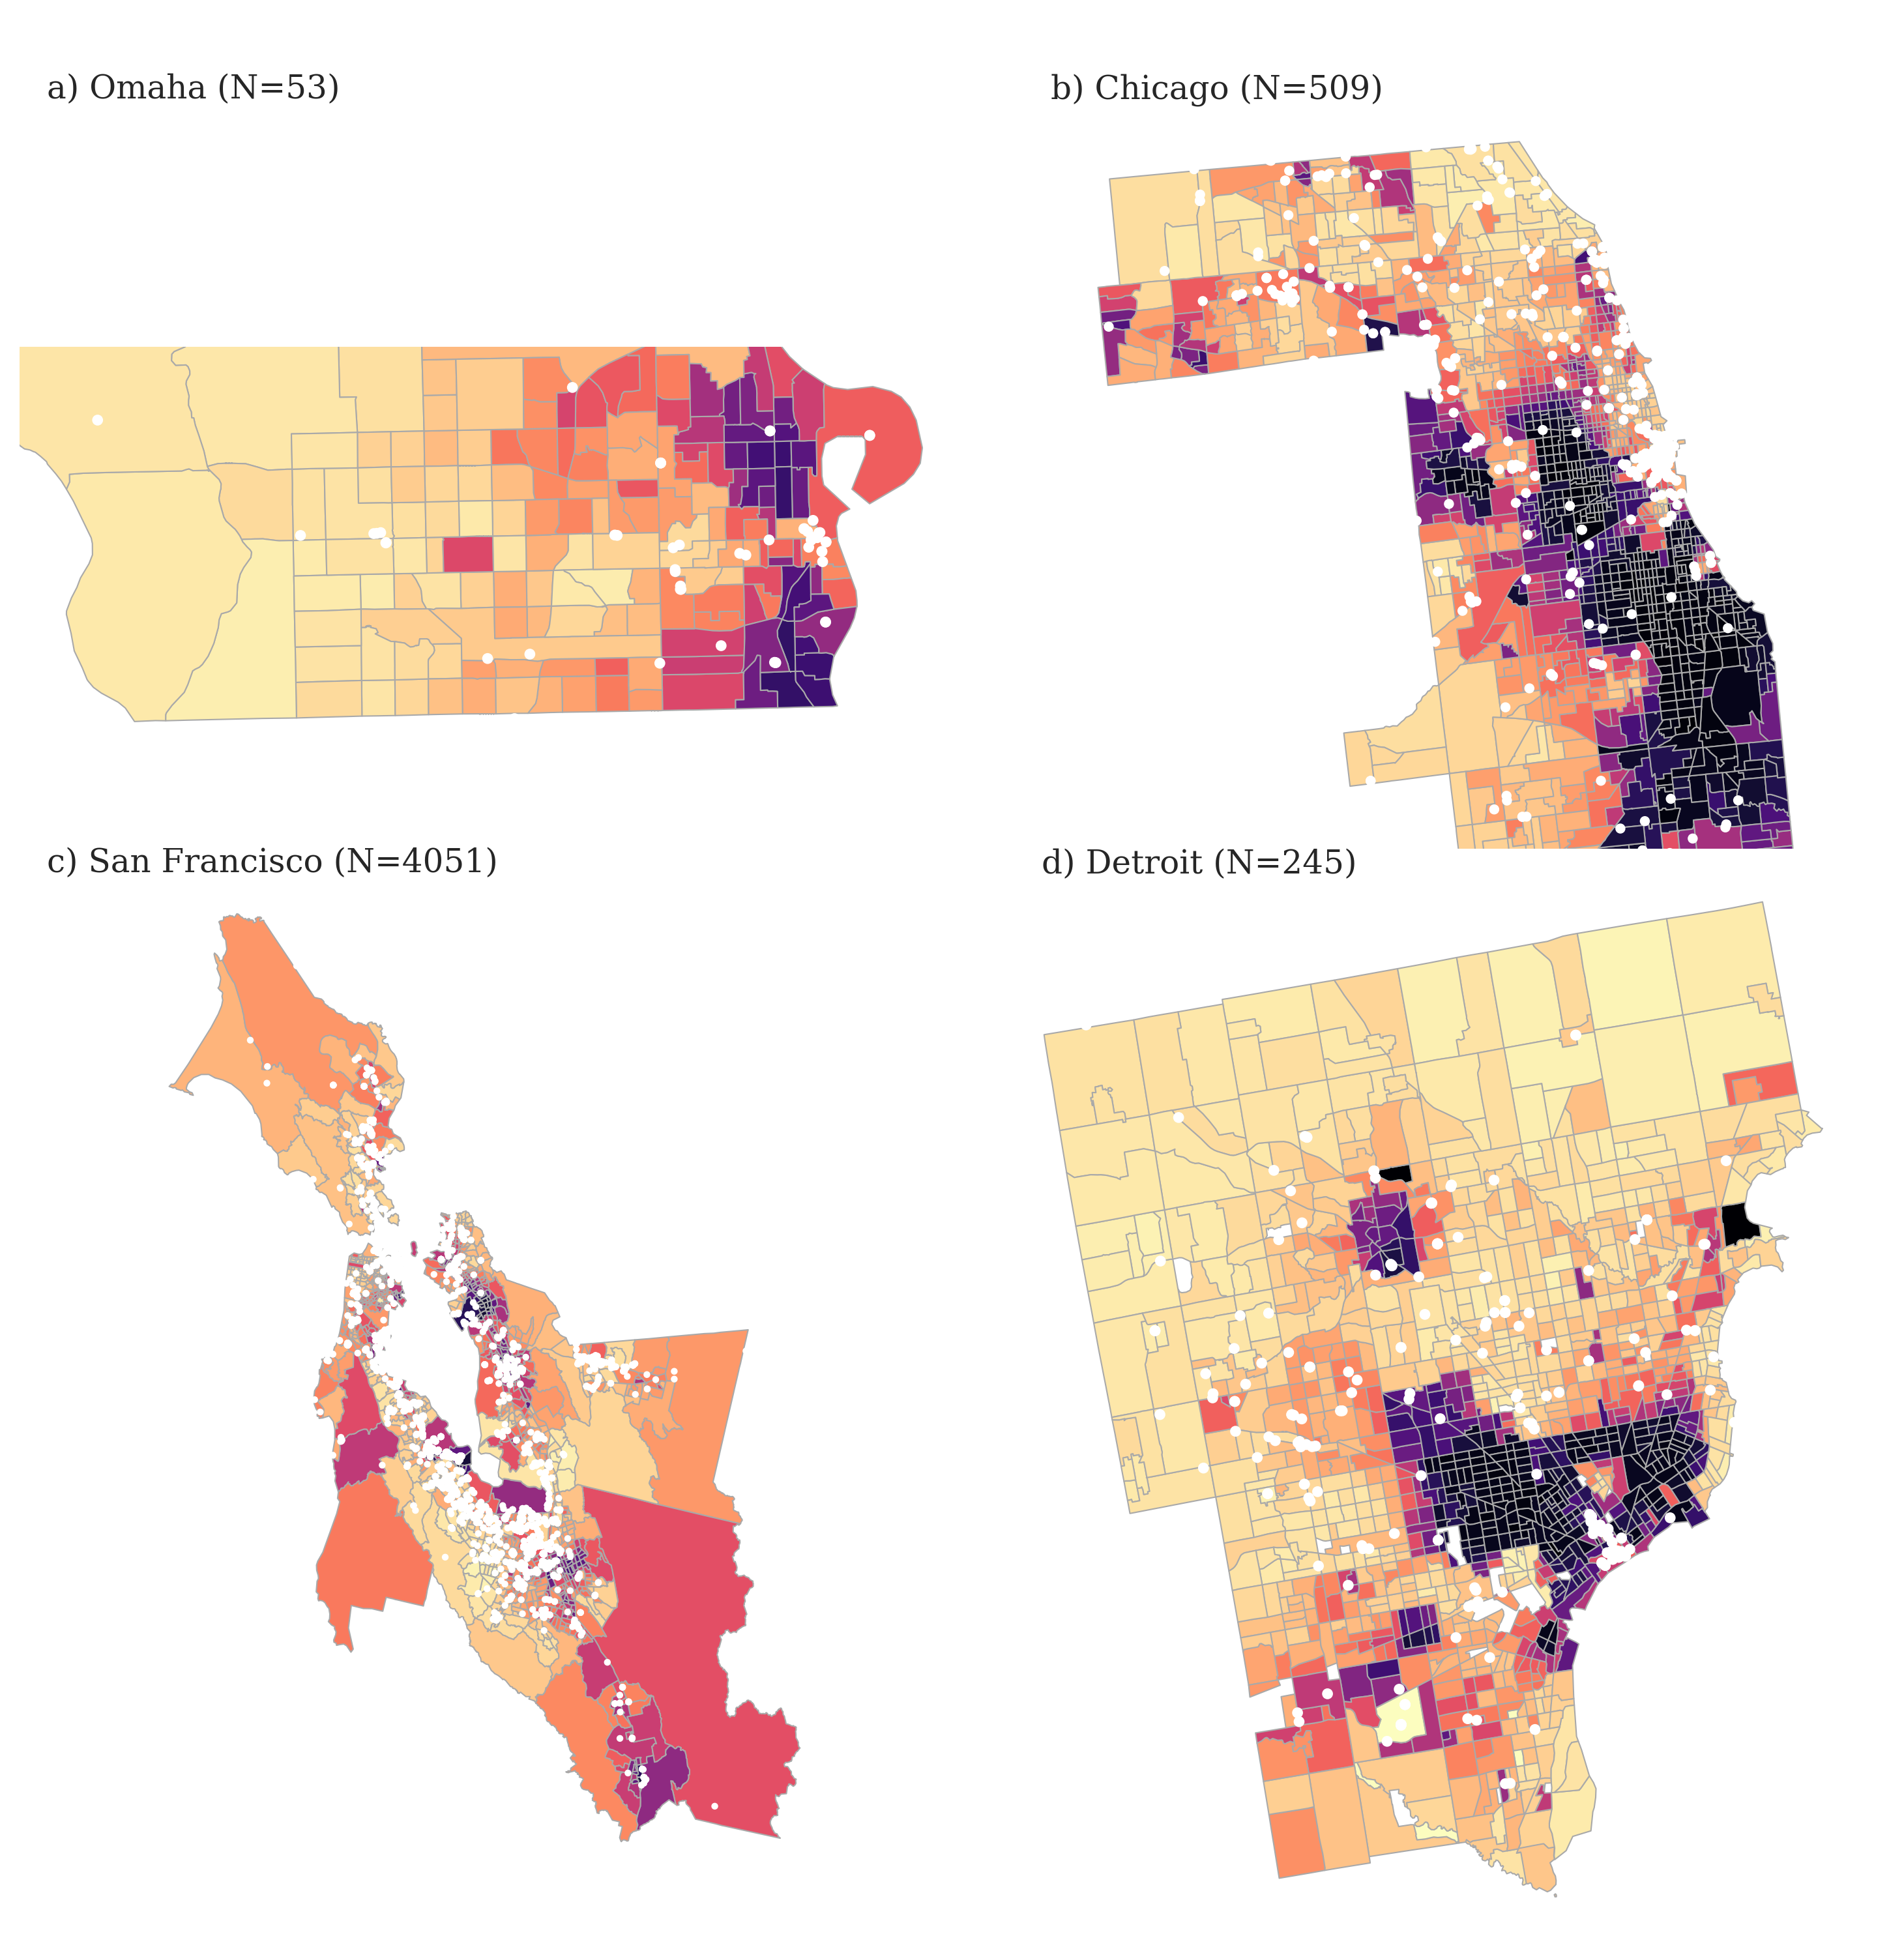
\includegraphics{TRB_2023_files/figure-pdf/fig-equity-output-1.png}

}

\caption{\label{fig-equity}Charging station locations for four
metropolitan regions}

\end{figure}

Another useful descriptive comparison between the PEV and charging
station markets is shown in Figure~\ref{fig-state-compare}. PEV sales
market share is plotted against charging stations per thousand residents
as of 2020. While there appears to be a positive correlation between
these infrastructures, there are clearly other factors at play - e.g.,
observe the difference between California and Vermont. This comparison
suggests that there are other factors that drive PEV adoption and it may
not be sufficient to simply install EVSE.

\begin{figure}

{\centering 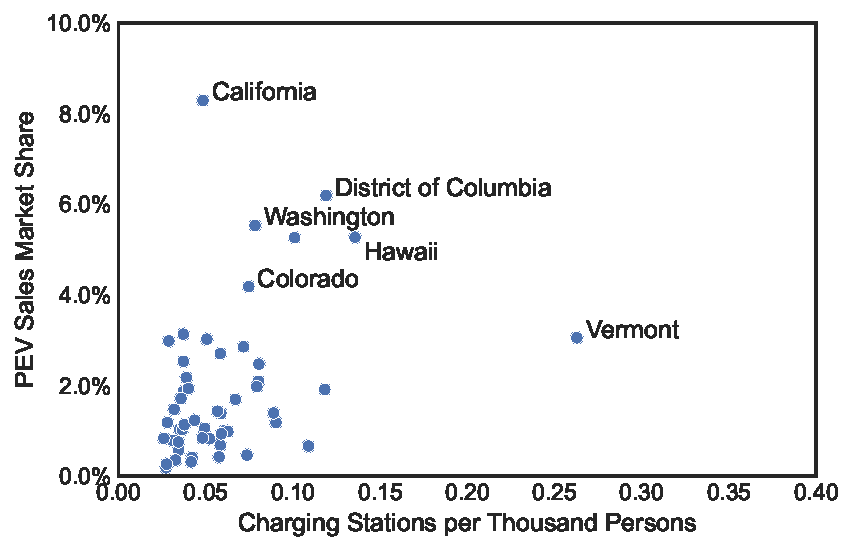
\includegraphics{TRB_2023_files/figure-pdf/fig-state-compare-output-1.pdf}

}

\caption{\label{fig-state-compare}Charging stations and PEV sales by
state in 2020}

\end{figure}

\hypertarget{phasing-causality}{%
\subsection{Phasing Causality}\label{phasing-causality}}

Before conducting the phasing causality tests, we applied Augmented
Dickey-Fuller (ADF) and Kwiatkouski-Phillips-Schmidt-Shin (KPSS) tests
for stationarity to the aggregated US time series and its first
differenced analogue. In both cases, it was found that the time series
is non-stationary. ADF and KPSS tests were also iteratively applied to
each county time series with similar results.

A limitation to the machine learning-based causality tests is that they
require large datasets to perform inference on a highly non-stationary
time series, as we found to be the case here. Five annual data points is
insufficient to run the tests. We overcome this barrier by leveraging
the spatio-temporal nature of our dataset. The strategy is to consider
each county as a slice of a spatio-temporal series. We select only the
2020 data and assume that charging stations and EV registrations in that
year may be affected by their corresponding observations in previous
years but not observations in other counties. This approach effectively
defines a spatio-temporal series with a maximum lag of four units
(lagged 2018, 2016, 2014, and 2012 observations) plus an instantaneous
effect (the 2020 observation). Figure~\ref{fig-lags} illustrates the
concept for five randomly selected counties.

\begin{figure}

{\centering 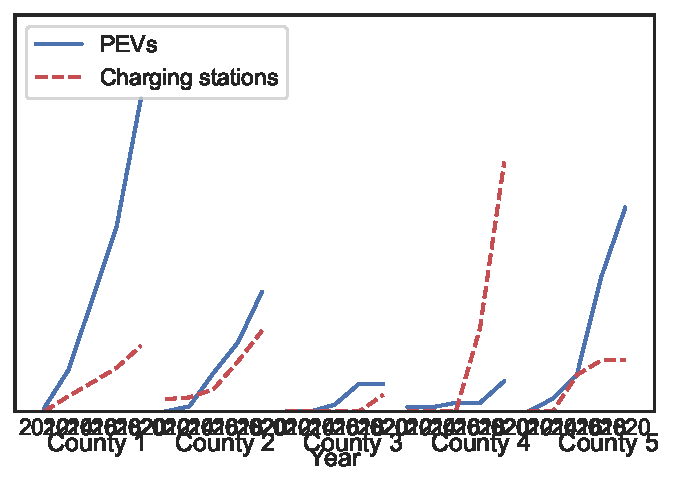
\includegraphics{TRB_2023_files/figure-pdf/fig-lags-output-1.pdf}

}

\caption{\label{fig-lags}Spatio-temporal lag illustration for five
random counties}

\end{figure}

We perform the non-linear causality tests using MLP, LSM, GRU, and ARIMA
models, with resulted summarized in (\textbf{tab-phasing-tests?}). Given
that charging station data can be aggregated to annual totals in every
year, we also test both one and two year lags alternatively considering
charging stations and EV registrations as the causal impetus. That is,
we consider 2012, 2014, 2016, 2018, and 2020 station totals and 2011,
2015, 2017, and 2019 station totals causing PEV registrations in the
five available years, then add 2021 station totals and consider PEV
registrations as causing charging station deployments. None of these
analyses gives definitive support for either causal mechanisms. These
results indicate a feedback relationship between the two variables of
interest. While our spatio-temporal approach allows us to perform these
statistical tests, it does not allow us to test for feedback effects
because the underlying time series remains too short.

Granger (Granger 1969) notes that the speed of information flow is an
important factor in causal phasing, as well as the data sampling
frequency. He suggests that results may differ depending upon if
analysis is conducted at an annual, quarterly, or monthly frequency.
However, the electric transportation market does not change fast enough
pace for sub-annual variation to be significant. Two pertinent factors
to consider are that vehicles tend to be kept for many years and a
single charging station is unlikely to incentive widespread EV purchases
in a county. As such, it is unlikely that individuals respond to
charging station investments at a sub-annual frequency and this
frequency is deemed acceptable.

\hypertarget{tab-phasing-tests}{}
\begin{longtable}[]{@{}llllll@{}}
\toprule()
Model & Lag & (1) & (2) & (3) & (4) \\
\midrule()
\endhead
ARIMA & 1 & 0.012 & 0.031 & 0.027 & 0.030 \\
ARIMA & 2 & 0.010 & 0.029 & 0.026 & 0.026 \\
ARIMA & 3 & 0.013 & 0.018 & 0.025 & 0.031 \\
ARIMA & 4 & 0.005 & 0.025 & 0.016 & 0.024 \\
ARIMA & 5 & 0.000 & 0.018 & 0.010 & 0.005 \\
GRU & 1 & 0.131 & 0.199 & 0.156 & 0.258 \\
LSTM & 1 & 0.240 & 0.231 & 0.133 & 0.035 \\
LSTM & 2 & 0.211 & 0.157 & 0.101 & 0.357 \\
LSTM & 3 & 0.196 & 0.069 & 0.145 & 0.062 \\
LSTM & 5 & 0.144 & 0.094 & 0.102 & 0.264 \\
MLP & 2 & 0.253 & 0.433 & 0.627 & 0.164 \\
MLP & 3 & 0.120 & 0.511 & 0.414 & 0.526 \\
MLP & 4 & 0.197 & 0.522 & 0.371 & 0.210 \\
MLP & 5 & 0.008 & 0.506 & 0.574 & 0.100 \\
NN & 1 & 0.160 & 0.007 & 0.003 & 0.136 \\
NN & 3 & 0.155 & 0.044 & 0.097 & 0.020 \\
NN & 4 & 0.053 & 0.064 & 0.036 & 0.049 \\
\bottomrule()
\end{longtable}

\hypertarget{gps-based-potential-outcomes-causality}{%
\subsection{GPS-Based Potential Outcomes
Causality}\label{gps-based-potential-outcomes-causality}}

Given the inconclusive phasing causality results, we maintain the
assumption that charging stations cause PEV registrations in subsequent
analysis. This section first presents the GPS model results that are
input into the GAM dose-response model. We then provide the
dose-response results, followed by mediation model results.

\hypertarget{gps-model-results}{%
\subsubsection{GPS Model Results}\label{gps-model-results}}

The GPS model includes spatially lagged charging stations per 100,000
persons in adjacent counties, the portion of the population that
identifies as a minority, median household income in \$10,000, and
state-year fixed effects (omitted from (\textbf{tab-gps-results?})). As
expected, we find that charging stations in adjacent counties are
correlated with more charging stations in the home county. Counties with
higher minority population shares tend to have lower charging station
access. Income is found to have a negative effect on charging station
access. At first glance, this is an unintuitive result because we tend
to see more amenities in higher income communities. A plausible reason
for this result is that higher income counties tend to have larger homes
in which residents can charge their vehicles, thus reducing the need for
public charging stations. As illustrated in Figure~\ref{fig-equity},
charging stations are concentrated in urban counties that tend to have
lower median incomes than their surrounding suburban counties. The pump
price parameter has the expected positive sign, indicative of more
charging stations when and where conventional fuel prices are high.

\hypertarget{tab-gps-results}{}
\begin{longtable}[]{@{}lll@{}}
\toprule()
~ & est. & t-stat \\
\midrule()
\endhead
Lagged charging stations & 0.019 & 13.05 \\
Percent minority & -8.2 & -1.42 \\
Household income (\$10,000) & -0.29 & -4.87 \\
Pump gas price (2020\$) & 3.7 & 1.07 \\
\bottomrule()
\end{longtable}

\hypertarget{dose-response-model-results}{%
\subsection{Dose-Response Model
Results}\label{dose-response-model-results}}

Figure~\ref{fig-dose-response} confirms the hypothesis that charging
station access encourages individuals to purchase PEVs. However, the
encouragement tends to become less effective at higher charging station
penetration rates. In fact, it becomes negative in the region around 100
charging stations per 100,000 persons when controlling for other
covariates. This result fits our finding in
Figure~\ref{fig-state-compare} that California has the highest PEV sales
market share despite several other states having more charging stations
per capita.

\begin{figure}

{\centering 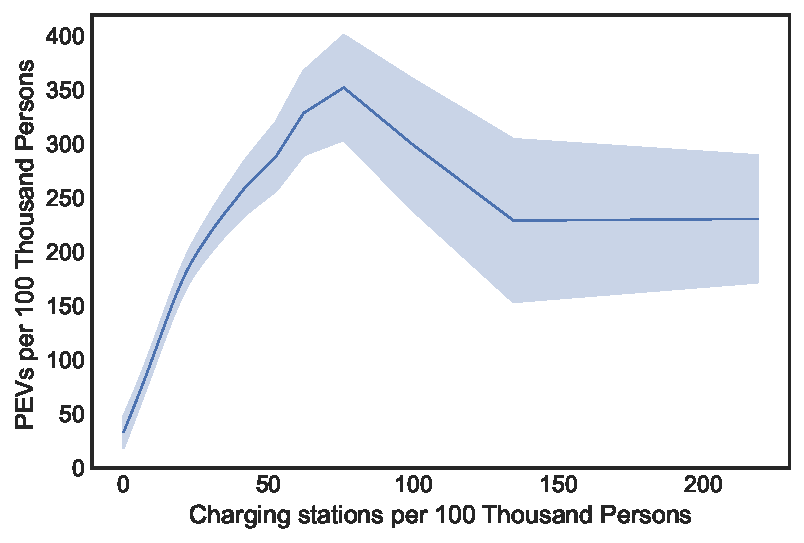
\includegraphics{TRB_2023_files/figure-pdf/fig-dose-response-output-1.pdf}

}

\caption{\label{fig-dose-response}Dose-response curve for charging
stations and PEV registrations}

\end{figure}

\hypertarget{mediation-effect-results}{%
\subsection{Mediation Effect Results}\label{mediation-effect-results}}

Mediation plots are shown in Figure~\ref{fig-med-co2} and
Figure~\ref{fig-med-elect} for grid CO\_2e intensity and Democratic vote
share, respectively. The mediation plots show the proportion of the
effect from each treatment variable that is caused by the mediating
effect of charging stations. In the case of CO\_2e emissions rate,
charging stations account for roughly 18\% of the effect for most
states. However, in the states with the highest emissions intensities
there are either very few registered PEVs (no effect from either
charging stations or grid CO\_2e intensity) or PEV registrations are
driven by charging stations investments despite a high CO2e emissions
intensity state grid. These results suggest that lowering grid emissions
tends to increase PEV registrations, but it is also feasible to
encourage minimal PEV adoption with a highly emitting grid via
investments in charging station infrastructure.

\begin{figure}

{\centering 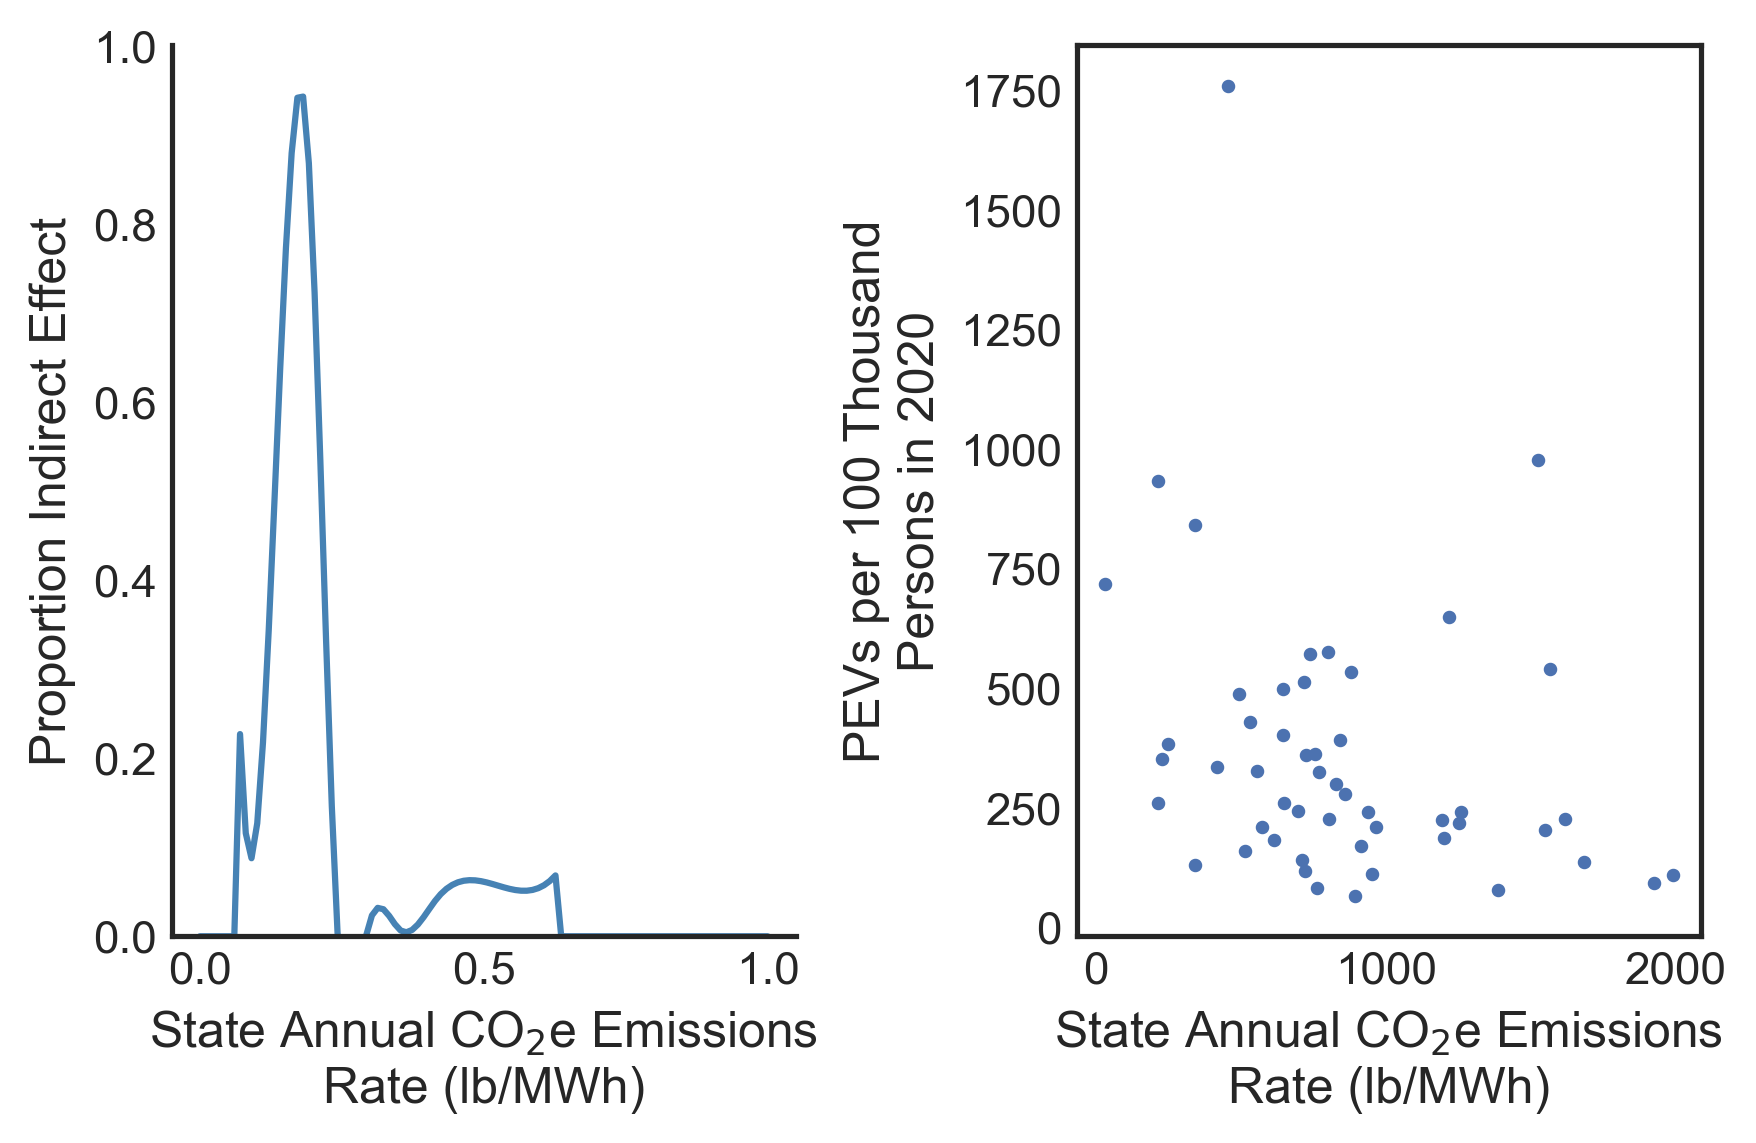
\includegraphics{TRB_2023_files/figure-pdf/fig-med-co2-output-1.png}

}

\caption{\label{fig-med-co2}Mediation results for CO2}

\end{figure}

Democratic vote share is mediated by EVSE infrastructure only in the
lowest share range. Similar to highly emitting grids, it appears that
EVSE investments can mediate the effect of political affiliation on PEV
registrations. However, the PEV adoption rates tend to be low in these
counties.

\begin{figure}

{\centering 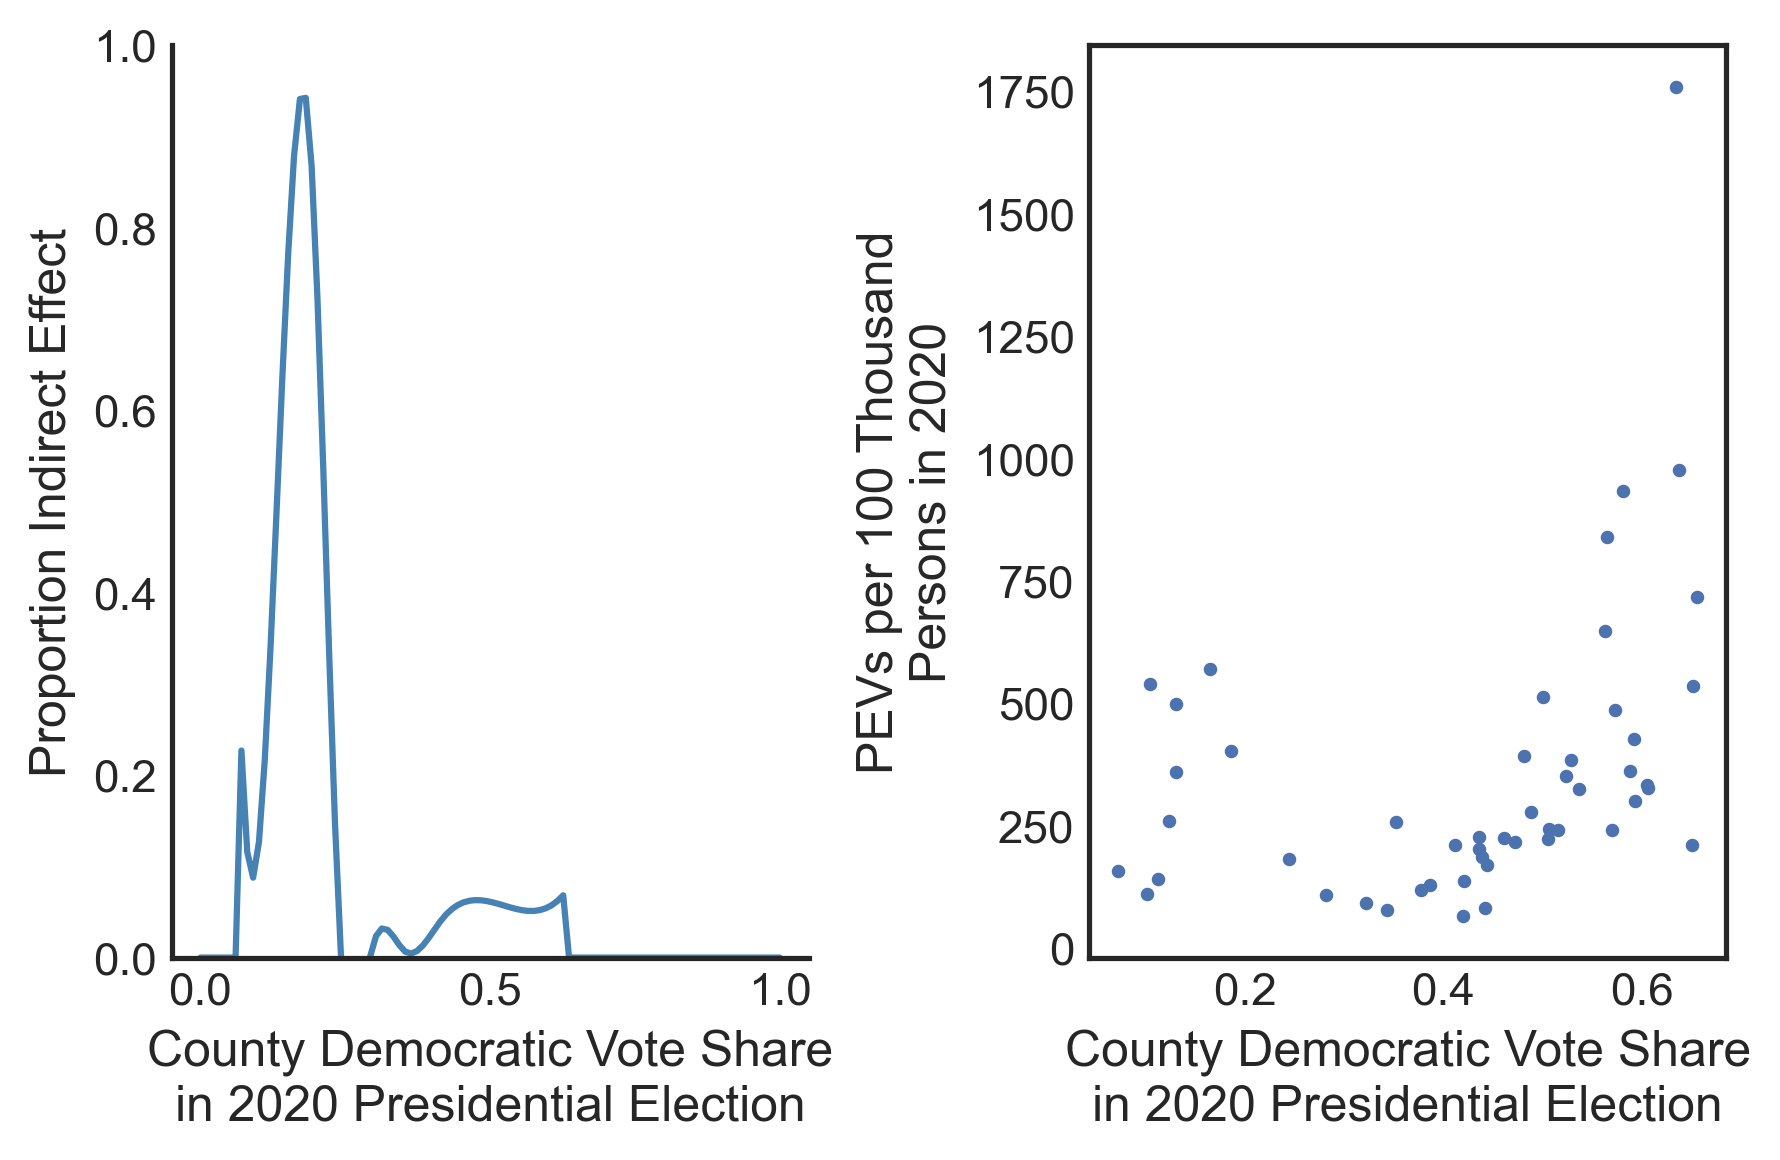
\includegraphics{TRB_2023_files/figure-pdf/fig-med-elect-output-1.png}

}

\caption{\label{fig-med-elect}Mediation results for 2020 presidential
election returns}

\end{figure}

\hypertarget{discussion-and-conclusions}{%
\section{Discussion and Conclusions}\label{discussion-and-conclusions}}

A key climate change policy challenge in the transportation sector is
how to transition the private vehicle fleet to PEVs. As in many product
markets, there is an indirect network effect between household goods
purchases and the supply of complementary infrastructure. Zhou and Li
(Zhou and Li 2018) found a critical mass hurdle may exist in the PEV
market, beyond which PEV sales may revert to a no-adoption outcome.
Their analysis was based on 2011-2013 data, which we are able to expand
upon by making use of an updated and longer time series. We find that
many US counties (239 out of 3273 as of 2020) have no registered PEVs
(measured as the number of battery-electric and plug-in hybrid electric
vehicles). Among those counties that have seen PEV adoption, there is a
clear pattern of concurrent charging station installations. We are
unable to confirm a causal phasing between the two actions using
non-linear Granger causality-type testing. It appears there is a
feedback relationship whereby PEVs are purchased and in response
suppliers install charging stations, and vice versa. There also appears
to be an equilibrium point, an ESCE penetration rate beyond which PEV
adoption does not increase absent supporting policies and incentives -
see the comparison between California and Vermont in
Figure~\ref{fig-state-compare}. Despite progress in some regions, PEV
adoption and EVSE infrastructure in most of the country is limited as of
2020. The high rate of zero valued observations in these datasets
suggests that PEV adoption and infrastructure networks are still more
concentrated. This concentration decreased in the time period of the
study, but still remained high in 2020.

In addition to the lack of findings from the causality models, the GPS
model returned significant findings on the affects of race on charging
station access. There is a correlation between counties with higher
representations of racial minorities and a lower rate of charging
stations. There were no significant findings on the effects of income.
The dose-response model finds that charging station access encourages
PEV adoption up until a certain point, then PEV adoption becomes
discouraged by increasing charging stations. Furthermore, the mediation
effect results, which studied grid emissions and Democratic voter share
per county, showed that both of these effects are mediated by charging
station infrastructure at higher levels of emissions and Democratic
voter share.

We find support for the Biden administration's focus on equitable
distribution of charging infrastructure within regions. Historically
segregated cities (e.g., Chicago and Detroit) lack EVSE in their
predominantly minority communities, while appearing to have an
overabundance of EVSE in their peripheral suburbs. There are also
inequities across regions. The Great Plains has very little charging
station infrastructure built, as seen by Omaha where EVSE is sparse
outside its downtown.

Several updates are proposed to the propensity score function. Despite
progress in some regions, PEV adoption and EVSE infrastructure in most
of the country is limited as of 2020. As such, there is a high
proportion of zero-valued observations. The linear GPS function could be
replaced by a Tobit specification, which would capture the zero
inflation as a censoring process. The current GPS function also treats
observations from the same county as independent. An autoregressive
specification could be explored that would match observations across
counties but treat sequential observations for the same county as a
common unit. Both changes are planned for a future iteration of this
work.

\hypertarget{refs}{}
\begin{CSLReferences}{1}{0}
\leavevmode\vadjust pre{\hypertarget{ref-aaa2022}{}}%
AAA. 2022. {``State Gas Price Averages.''}
\url{https://gasprices.aaa.com/state-gas-price-averages/}.

\leavevmode\vadjust pre{\hypertarget{ref-adepetu2017}{}}%
Adepetu, Adedamola, and Srinivasan Keshav. 2017. {``The Relative
Importance of Price and Driving Range on Electric Vehicle Adoption: Los
Angeles Case Study.''} \emph{Transportation} 44 (2): 353--73.
\url{https://doi.org/10.1007/s11116-015-9641-y}.

\leavevmode\vadjust pre{\hypertarget{ref-aultman-hall2018}{}}%
Aultman-Hall, Lisa. 2018. {``Incorporating Long-Distance Travel into
Transportation Planning in the United States.''}
\url{https://escholarship.org/uc/item/0ft8b3b5}.

\leavevmode\vadjust pre{\hypertarget{ref-diamond2009}{}}%
Diamond, David. 2009. {``The Impact of Government Incentives for
Hybrid-Electric Vehicles: Evidence from US States.''} \emph{Energy
Policy} 37 (3): 972--83.
\url{https://doi.org/10.1016/j.enpol.2008.09.094}.

\leavevmode\vadjust pre{\hypertarget{ref-eia2022}{}}%
EIA. 2022. {``Retail Prices for Gasoline.''}
\url{https://www.eia.gov/dnav/pet/pet_pri_gnd_a_epm0_pte_dpgal_a.htm}.

\leavevmode\vadjust pre{\hypertarget{ref-elfalan2021}{}}%
Elfalan, Jonathan. 2021. {``Electric Car Range and Consumption.''}
\url{https://www.edmunds.com/car-news/electric-car-range-and-consumption-epa-vs-edmunds.html}.

\leavevmode\vadjust pre{\hypertarget{ref-elhorst2017}{}}%
Elhorst, J Paul, and Solmaria Halleck Vega. 2017. {``The SLX Model:
Extensions and the Sensitivity of Spatial Spillovers to W.''}
\emph{Papeles de Economía Española} 152: 34--50.

\leavevmode\vadjust pre{\hypertarget{ref-epa2021}{}}%
EPA, US. 2021. {``Inventory of u.s. Greenhouse Gas Emissions and Sinks:
1990-2019.''}
\url{https://www.epa.gov/ghgemissions/inventory-us-greenhouse-gas-emissions-and-sinks}.

\leavevmode\vadjust pre{\hypertarget{ref-galagate2016}{}}%
Galagate, Douglas. 2016. {``Causal Inference with a Continuous Treatment
and Outcome: Alternative Estimators for Parametric Dose-Response
Functions with Applications.''} PhD thesis.

\leavevmode\vadjust pre{\hypertarget{ref-granger1969}{}}%
Granger, Clive. 1969. {``Investigating Causal Relations by Econometric
Models and Cross-Spectral Methods.''} \emph{Econometrica} 37 (3): 16.

\leavevmode\vadjust pre{\hypertarget{ref-hidrue2011}{}}%
Hidrue, Michael K., George R. Parsons, Willett Kempton, and Meryl P.
Gardner. 2011. {``Willingness to Pay for Electric Vehicles and Their
Attributes.''} \emph{Resource and Energy Economics} 33 (3): 686--705.
\url{https://doi.org/10.1016/j.reseneeco.2011.02.002}.

\leavevmode\vadjust pre{\hypertarget{ref-hirano2005}{}}%
Hirano, Keisuke, and Guido W. Imbens. 2005. {``The Propensity Score with
Continuous Treatments.''} In, edited by Andrew Gelman and Xiao-Li Meng,
73--84. Chichester, UK: John Wiley \& Sons, Ltd.
\url{https://doi.org/10.1002/0470090456.ch7}.

\leavevmode\vadjust pre{\hypertarget{ref-imai2009}{}}%
Imai, Susumu, Neelam Jain, and Andrew Ching. 2009. {``Bayesian
Estimation of Dynamic Discrete Choice Models.''} \emph{Econometrica} 77
(6): 1865--99. \url{https://doi.org/10.3982/ECTA5658}.

\leavevmode\vadjust pre{\hypertarget{ref-itf2021}{}}%
ITF. 2021. {``Transport Outlook 2021.''} Paris.
\url{https://www.oecd-ilibrary.org/transport/per-capita-demand-for-urban-passenger-transport-by-world-region-to-2050_097a0f3e-en}.

\leavevmode\vadjust pre{\hypertarget{ref-kobrosly2020}{}}%
Kobrosly, Roni W. 2020. {``Causal-Curve: A Python Causal Inference
Package to Estimate Causal Dose-Response Curves.''} \emph{Journal of
Open Source Software} 5 (52): 2523.
\url{https://doi.org/10.21105/joss.02523}.

\leavevmode\vadjust pre{\hypertarget{ref-larson2021}{}}%
Larson, E., C. Greig, J. Jenkins, E. Mayfield, A. Pascale, C. Zhang, J.
Drossman, et al. 2021. {``Net-Zero America: Potential Pathways,
Infrastructure, and Impacts, Final Report.''} Princeton, NJ.
\url{https://netzeroamerica.princeton.edu/the-report}.

\leavevmode\vadjust pre{\hypertarget{ref-li2017}{}}%
Li, Shanjun, Lang Tong, Jianwei Xing, and Yiyi Zhou. 2017. {``The Market
for Electric Vehicles: Indirect Network Effects and Policy Design.''}
\emph{Journal of the Association of Environmental and Resource
Economists} 4 (1): 89--133. \url{https://doi.org/10.1086/689702}.

\leavevmode\vadjust pre{\hypertarget{ref-melliger2018}{}}%
Melliger, Marc A., Oscar P. R. van Vliet, and Heikki Liimatainen. 2018.
{``Anxiety Vs Reality {\textendash} Sufficiency of Battery Electric
Vehicle Range in Switzerland and Finland.''} \emph{Transportation
Research Part D: Transport and Environment} 65 (December): 101--15.
\url{https://doi.org/10.1016/J.TRD.2018.08.011}.

\leavevmode\vadjust pre{\hypertarget{ref-menendian2020}{}}%
Menendian, Stephen, Samir Gambhir, and Chih-Wei Hsu. 2020. {``Roots of
Structural Racism.''}

\leavevmode\vadjust pre{\hypertarget{ref-musti2011}{}}%
Musti, Sashank, and Kara M. Kockelman. 2011. {``Evolution of the
Household Vehicle Fleet: Anticipating Fleet Composition, PHEV Adoption
and GHG Emissions in Austin, Texas.''} \emph{Transportation Research
Part A: Policy and Practice} 45 (8): 707--20.
\url{https://doi.org/10.1016/J.TRA.2011.04.011}.

\leavevmode\vadjust pre{\hypertarget{ref-rosol2022}{}}%
Rosoł, Maciej, Marcel Młyńczak, and Gerard Cybulski. 2022. {``Granger
Causality Test with Nonlinear Neural-Network-Based Methods: Python
Package and Simulation Study.''} \emph{Computer Methods and Programs in
Biomedicine} 216 (April): 106669.
\url{https://doi.org/10.1016/j.cmpb.2022.106669}.

\leavevmode\vadjust pre{\hypertarget{ref-rubin2005}{}}%
Rubin, Donald B. 2005. {``Causal Inference Using Potential Outcomes:
Design, Modeling, Decisions.''} \emph{Journal of the American
Statistical Association} 100 (469): 322--31.
\url{https://doi.org/10.1198/016214504000001880}.

\leavevmode\vadjust pre{\hypertarget{ref-sheldon2019}{}}%
Sheldon, Tamara L., J. R. DeShazo, and Richard T. Carson. 2019.
{``Demand for Green Refueling Infrastructure.''} \emph{Environmental and
Resource Economics} 74 (1): 131--57.
\url{https://doi.org/10.1007/s10640-018-00312-9}.

\leavevmode\vadjust pre{\hypertarget{ref-silvia2016}{}}%
Silvia, Chris, and Rachel M. Krause. 2016. {``Assessing the Impact of
Policy Interventions on the Adoption of Plug-in Electric Vehicles: An
Agent-Based Model.''} \emph{Energy Policy} 96 (September): 105--18.
\url{https://doi.org/10.1016/J.ENPOL.2016.05.039}.

\leavevmode\vadjust pre{\hypertarget{ref-spieler2020}{}}%
Spieler, Christof. 2020. {``Racism Has Shaped Public Transit, and It{'}s
Riddled with Inequities.''}
\url{https://kinder.rice.edu/urbanedge/2020/08/24/transportation-racism-has-shaped-public-transit-america-inequalities}.

\leavevmode\vadjust pre{\hypertarget{ref-sullivan2021}{}}%
Sullivan, Brian, and Harriet Taylor. 2021. {``The u.s. EV Charging
Network Isn't Ready for Your Family Road Trip, Let Alone the Expected
Wave of New Cars.''}
\url{https://www.cnbc.com/2021/08/24/cnbc-road-test-the-us-ev-charging-network-isnt-ready-for-your-family-road-trip-let-alone-the-expected-wave-of-new-cars.html}.

\leavevmode\vadjust pre{\hypertarget{ref-thewhitehouse2021-a}{}}%
The White House. 2022. {``The Biden-Harris Electric Vehicle Charging
Action Plan.''}
\url{https://www.whitehouse.gov/briefing-room/statements-releases/2021/12/13/fact-sheet-the-biden-harris-electric-vehicle-charging-action-plan/}.

\leavevmode\vadjust pre{\hypertarget{ref-uscensusbureau2020}{}}%
US Census Bureau. 2020. {``Inequalities Persist Despite Decline in
Poverty for All Major Race and Hispanic Origin Groups.''}
\url{https://www.census.gov/library/stories/2020/09/poverty-rates-for-blacks-and-hispanics-reached-historic-lows-in-2019.html}.

\leavevmode\vadjust pre{\hypertarget{ref-vehicletechnologyoffice2022}{}}%
Vehicle Technology Office. 2022. {``More Than Half of All Daily Trips
Were Less Than Three Miles in 2021.''}
\url{https://www.energy.gov/eere/vehicles/articles/fotw-1230-march-21-2022-more-half-all-daily-trips-were-less-three-miles-2021}.

\leavevmode\vadjust pre{\hypertarget{ref-wolbertus2018}{}}%
Wolbertus, Rick, Maarten Kroesen, Robert van den Hoed, and Caspar G.
Chorus. 2018. {``Policy Effects on Charging Behaviour of Electric
Vehicle Owners and on Purchase Intentions of Prospective Owners: Natural
and Stated Choice Experiments.''} \emph{Transportation Research Part D:
Transport and Environment} 62 (July): 283--97.
\url{https://doi.org/10.1016/j.trd.2018.03.012}.

\leavevmode\vadjust pre{\hypertarget{ref-zhou2018}{}}%
Zhou, Yiyi, and Shanjun Li. 2018. {``Technology Adoption and Critical
Mass: The Case of the U.S. Electric Vehicle Market: Technology Adoption
and Critical Mass.''} \emph{The Journal of Industrial Economics} 66 (2):
423--80. \url{https://doi.org/10.1111/joie.12176}.

\end{CSLReferences}



\end{document}
